\documentclass[12pt]{article}
\usepackage[utf8]{inputenc}
\usepackage[top=20mm,bottom=20mm,left=25mm,right=25mm]{geometry}
\usepackage[style=phys,url=false,doi=false,isbn=false,eprint=false]{biblatex}
\usepackage[skip=1em,indent=0em]{parskip}
\usepackage{amsmath}
\usepackage{graphicx}
\usepackage{hyperref}
\usepackage{cleveref}
\usepackage{physics}
\usepackage{siunitx}
\usepackage{lipsum}
\usepackage{xurl}
\usepackage{caption}
\usepackage{subcaption}
\usepackage{float}
\usepackage{tikz}
\usepackage{amsfonts}

\addbibresource{bibliographies/Background.bib}
\addbibresource{bibliographies/bib2.bib}
\addbibresource{bibliographies/bib3.bib}
\addbibresource{bibliographies/bib4.bib}
\addbibresource{bibliographies/bib6.bib}
\addbibresource{bibliographies/bibLOQC.bib}
\addbibresource{bibliographies/Introduction.bib}
\addbibresource{bibliographies/TrappedIonQC.bib}

% Macros for the 0 and 1 kets, might be a useful shorthand, if you want to use it just do \kz or \ko anywhere
\newcommand{\kz}{$\ket{0}$ }
\newcommand{\ko}{$\ket{1}$ }

\begin{document}
% \begin{center}
%     \Huge \textbf{How to build a Quantum Computer}
% \end{center}

% \begin{center}
%     \emph{\large All of us}
% \end{center}

% \title{How to buil a Quantum Computing}
% \author{All of us}

% \maketitle

% \tableofcontents

\pagestyle{empty}                       % No numbers on title page      

\par\noindent\includegraphics[width=12cm]{images/PandA_crest.pdf}

\par\noindent                                           % Centre Title, and name
\vspace*{2cm}
\begin{center}
        \Large\bf \Large\bf Group Project Report\\
        \LARGE\bf How to Build a Quantum Computer
        %Studying magnetic and structural properties of CoCl2 % Replace with your title
\end{center}
\vspace*{0.5cm}
\begin{center}
        \bf All of us\\                               % Replace with your name and
        February 2023                              % Submission Date
\end{center}
\vspace*{5mm}
%

\vspace*{1cm}

%\subsubsection*{Declaration}

% \begin{quotation}
%   I declare that this project and report is my own work.
% \end{quotation}

\vspace*{2cm}
%Signature:
         % You can include a scanned version 
                                                 % of you signature here, or comment 
                                                 % this line out

\vfill
{\bf Supervisor:} Dr. Gavin Woolman \hspace*{5cm}Date:  06/02/2023            % Change to suit
% \hfill
% 10 Weeks                                         % Change to suit
\newpage
%
%                       End of Title Page
\pagestyle{plain}                               % Page numbers at bottom
\setcounter{page}{1}                            % Set page number to 1
\tableofcontents                                % Makes Table of Contents

\section{Introduction}
A quantum computer uses quantum mechanical phenomena to perform calculations which any classical computer, including supercomputers, would be unable to compute within a lifetime. \cite{noauthor_what_nodate}
This report will explain the physical process and technologies behind building such a machine. Initially, we provide the motivation for wanting to build a quantum computer, which will be followed by an overview of the progress made in both industry and academic research. In order to understand the complex methods used to construct a quantum computer, the report provides explanations of the basic fundamentals of classical computing and the key quantum mechanical concepts, such as entanglement and superposition. Then, we explore a current method for implementing quantum computers - trapped ions, before looking into the next possible breakthrough in the field with linear optical quantum computers.

\subsection{Why Build a Quantum Computer?}\label{sec:why}
In order to understand the power of quantum computers, it is helpful to look to cryptography for an example. Most of computer security in the late 20th and early 21st century has been underpinned by RSA encryption. In the simplest terms, RSA encrypted data has some number, $P$, associated with it, which is a semiprime - it is the product of two prime factors. If you can determine these two factors then you can decrypt the data. If you know one of the factors then it is very easy to find the other, simply by dividing $P$ by the known factor. However, even with some holistic assumption and simplification there is no mathematical formula to compute both factors without any prior knowledge. Therefore, it becomes a case of trial and error which is trivial for a small number such as 15, as you quickly find 5 and 3. However, for a semiprime such as 403135, there are a many more possible factors to trial. In fact, modern RSA encryption uses semiprimes comprising over 1000 digits.

A typical classical computer with $n$ bits can represent $2^n$ different values, so in theory could trial $2^n$ factors. It would process each trial value sequentially. If we take the computation time for trialling one value to be constant, then the entire processing time scales as $2^n$. Therefore, for RSA encryption using significantly large semiprimes, the vast number of factors necessary to trial makes the computation time so long that the the encrypted data is effectively secure. It would take a classical computer 300 trillion years to trial all possible factors necessary to break RSA encryption using a semiprime of approximately 600 digits, as you would need a classical computer with 112 bits \cite{mahto2016security}\cite{quintessencelabs_2022}.
made 
This is where a quantum computer comes in. A quantum computer with $n$ qubits (quantum bits) can also represent $2^n$ different values, however, it can do so simultaneously. This is possible because of quantum mechanical phenomena such as superposition. If a quantum computer can try all possible factors at once, the processing time is now a constant. Therefore, a 112 qubit quantum computer could, in constant time, break the 600 bit RSA encryption that would take a classical computer 300 trillion years to solve.

This incredible processing power makes quantum computers ideal at solving many other combinatorics based problems, where finding the solution involves trying a vast number of possibilities. Two particularly interesting applications are in financial and medical simulation. Monte Carlo simulation calculates the likely outcome of a certain event by running enough simulations that it covers a suitable range of possibilities; these repeated simulations are equivalent to trialling different factors for RSA encryption. Goldman Sachs has invested heavily in this technology, and executed a quantum version of its Monte Carlo simulation on a trapped ion computer - they believe it will allow traders to obtain up-to-date risk predictions 10 times faster within the next five years \cite{Giurgica_Tiron_2022}. Quantum computers also have the potential to rapidly advance drug development by allowing researchers to test many different combinations of atoms and molecules simultaneously \cite{bova2021commercial}.

If you want a computer to watch YouTube or write a word processing document, then a quantum computer probably isn't necessary for you. However, if you want to accelerate humanity's innovation in medicine, physics, finance, cybersecurity and more, hopefully it's now clear why you should build a quantum computer.

\subsection{Current Methods of Quantum Computing}
There are multiple method to building a quantum computer and no single method is the leading approach.
Superconducting qubits (qubits are the quantum realisation of classical bits) is the method currently being researched by IBM, Google and a select few others and it was the first method to claim quantum supremacy. \cite{gibney_hello_2019}
Quantum supremacy is a term used to describe when a quantum computer is able to complete a calculation that a classical computer could not achieve in a reasonable amount of time. 

Google was first to claim it in 2019 with their 53 bit `Sycamore' quantum computer which reportedly solved a problem in under 5 hours which would take a classical computer over $10\text{ }000$ years \cite{gibney_hello_2019}.
However these claims were disputed by IBM - another large company heavily invested in the quantum computing race.
The largest quantum computer to date is the IBM osprey with 433 qubits announced in November 2022 \cite{irving_ibm_2022}.

This report will instead focus on trapped ion systems. 
One of the largest contenders in this area is IonQ with a 23 qubit computer. 
 Although trapped ions systems have not yet reached the number of qubits as seen from superconducting systems there are many advantages such as: 
\begin{itemize}
    \item The cost of ion trap systems is relatively low - therefore research can be carried out by academics and be peer-reviewed. As opposed to superconducting systems which require vast investments, leading to only a select few companies willing to research this approach. Therefore significantly more detailed research is available on ion trapped systems.  
    \item Many small (tens of qubits) quantum computers have been built using trapped ion systems. It fulfils all the requirements for a quantum computer however it is a difficult to scale to hundreds of qubits. See section \ref{sec:Trapped}
    \item The company IonQ produces commercially available quantum computer using trapped ion systems which can be accessed from public clouds such as Microsoft Azure. \cite{sonialopezbravo_ionq_nodate} Goldman Sachs have been using this service to test quantum algorithms relevant to the financial services industry. \cite{noauthor_goldman_2021}
\end{itemize}




The next section in this report will provide some background information and explain some key fundamential ideas in classical computing and quatum information. 
The following section will then venture into trapped ion systems where quantum computers have been built using this method.
It will cover how physical qubits are created and manipulated using gates for calculations to be carried out and finally how the qubit states can be readout. 


Lastly the report will discus optical qubits due to their likely scalability for the future. 
Quantum computers are likely to require up to millions of qubits for most quantum algorithms - as compared to the current record of 433 qubtis from IBM. \cite{bergou_quantum_2021} 
Optical qubits currently have some large hurdles to overcome - as will be discussed in section \ref{sec:Photonic}. 
However once these are overcome it is likely to be an attractive attender for future quantum computing and information transfer.
In particular, photons can maintain entanglement over long distances and time periods allowing secure transition of quantum information - this has been demonstrated for over 1200km. \cite{yin_satellite-based_2017}
\newpage
\section{Background}

\subsection{Quantum}
\subsubsection{Superposition}
Superposition is a uniquely quantum mechanical phenomenon where an object may exist in multiple states at once. 
For example an electron may be said to be in two places at once - or more accurately its probability function covers multiple areas in space. \cite{noauthor_whatCal_nodate}

Superposition can be observed in the polarisation of light. 
Light can be horizontally, vertically and circularly polarized and much of the light around us is a superposition of the three.
However when light interacts with surfaces their properties can change such as light reflecting off a pond being horizontally polarized. 
Using a linear polariser one can control the direction of polarisation of the light passing through it.
Constructing two polarisers at right angles (vertical and horizontal respectively) one would expect only vertical polarised light to emitted from the first and then no light to be emitted from the second polariser. 
This is what is experimentally observed - however if a third polariser is placed between the horizontal and vertical polarisers orientated at 45$^\circ$ (as in figure \ref{fig:polarisers}) from both then light will now be transmitted through the final horizontal polariser (at 50$\%$ intensity). \cite{noauthor_whatCal_nodate}
!!! make the link to superposition clearer here!!!

\begin{figure}[H]
  \centering
  \begin{subfigure}[b]{0.44\linewidth}
    \includegraphics[width=\linewidth]{images/2 polariser.jpg}
    \caption{Unpolarised light passing through a horizontal and then failing to pass through a vertical polarising filter. }\label{fig:2 polarise}
  \end{subfigure}
  \begin{subfigure}[b]{0.44\linewidth}
    \includegraphics[width=\linewidth]{images/3 polariser.jpg}
    \caption{Unpolarised light passing through three successive polarising filters. A horizontal and vertical filter and a linear polariser orientated 45$^\circ$ between both. }\label{fig:3 polarise}
  \end{subfigure}
  \caption{Unpolarised light passing through linear polarising filters in two set ups. \cite{noauthor_whatCal_nodate}}
  \label{fig:polarisers}
\end{figure}

\subsubsection{Entanglement}
Entanglement is when the measurement of one particles state will effect the state of another particle.
I.e. for interacting states A and B their combined wavefunction cannot be expressed as the product of the individual wavefunction's of A and B if states A and B are entangled. \cite{bransden_quantum_2000}
$\psi(A,B)\neq \psi(A)\cdot \psi(B)$ 



\subsection{The DiVincenzo Criteria -- to be polished}
The DiVincenzo criteria is a set of objectives that must be met for the physical realisation of a quantum computer. 
It sets out five basic principles which must met to build a functional quantum computer and two more principles for quantum information networks. \cite{bergou_quantum_2021}
This report focuses on the implementation of a single quantum computer and therefore focused on the first five principles.
The principles are:
\begin{enumerate}
    \item Scalability with well defined qubits
    \item The ability to initialise the system in a well defined, determinate state
    \item The ability to read out qubit state with high accuracy
    \item A set of universal quantum gates
    \item Long relevant decoherence times
    \newcounter{enumTemp}
    \setcounter{enumTemp}{\theenumi}
\end{enumerate}
The two principles for the implementation of quantum information networks are:
\begin{enumerate}
    \setcounter{enumi}{\theenumTemp}
    \item The ability to convert between `stationery' and `flying' qubits
    \item The ability to transmit flying qubits between specified locations
\end{enumerate}

There are various physical approaches for quantum computing that satisfy some of the DiVincenzo criteria, however no current approach has successfully satisfied all five.
\vspace{1em}

The first objective to implement well defined qubits which are saliable. An example of a well defined qubit is superposition of vertical and horizontal polarisation of a photons, or the spin up and spin down of electrons. 
There are many methods of creating well defined qubits, however scalability and producing multiple which remain in a superposition state is challenging.
IBM claimed in 2021 to have created the worlds largest quantum processor, the 127 qubit Eagle. \cite{authorfullname_ibm_nodate}
\vspace{1em}

The second objective is to initialise the qubits into a well defined determinate state i.e. initialise the qubit register so all are in the 0 state $\vert 0\rangle \vert 0\rangle$...$\vert 0 \rangle$. \cite{lapierre_divincenzo_2021}
\vspace{1em}

The third objective is to read out qubit state $\vert 0\rangle$ or $\vert 1 \rangle$ with high accuracy. 
This is a challenge with photons as a method for detecting individual photons with no dark count (false positives) does not exist yet.
\vspace{1em}

The fourth objective is to implement a universal set of gates, all operations can be preformed using two quantum gates.
One is gate which flips the state of a single qubit. The other is a CNOT gate which acts on two qubits and flips the state of one qubit only if the 'control' qubit is in state $\vert 1 \rangle$. \cite{lapierre_divincenzo_2021} 
\vspace{1em}

The final objective is for long `relevant' decoherence times, this requires the qubit to stay in a superposition quantum state for longer than the duration of gate operations before the state collapses. 

\newpage

\section{Trapped Ion Quantum Computing} \label{sec:Trapped}
In this section we provide an introduction to the implementation details of trapped ion quantum computers (**once done possibly elaborate what exactly we cover).
The qubits in a trapped ion system are represented by individual trapped ions.
As would have been seen in a quantum mechanics class, electrons bound in atoms can occupy a certain number of possible quantum states, here 2 of these level are chosen and used as the \kz and \ko states.
Though it isn't quite as simple as that, for quantum computing we must have a way of entangling these 2 states.
To achieve that, the qubit ions are trapped in the same trap and their motion within it is coupled as a quantum system, through which entanglement is achieved.
The rest of the required features for quantum computing including state preparation, readout and quantum gates are all achieved through tuned lasers (we use the word a bit loosely, it is to mean any source of a particular type of light) and or the mentioned entanglement.
The section is largely based on the review by Brunzewicz \cite{bruzewiczTrappedionQuantumComputing2019} and for a more detailed review on the subject we recommend that.

\subsection{Ion Trapping and the Paul Trap}
Ion trapping is an extensive field of expertise used for many purposes across physics and other sciences, it is an essential component of many devices and experiments that try to manipulate individual particles, molecules or so on.
For a brief sketch of what this involves, these experiments must be done in vacuum (otherwise there would be too many other atoms around) and rely on complex electric and magnetic fields to manipulate the motion of charged atoms.
For quantum computing we are interested in trapping individual ions in a stable way, and while we want to trap multiple of them (currently about 5-100 has been achieved \cite{paganoCryogenicTrappedionSystem2018}) it is important that we can tell them apart (as opposed to trapping them in bunches as is often done).

There are currently 2 dominant, suitable classes of ion traps, Penning traps which uses a combination of magnetic and electric fields, and Paul traps (also known as Quadrupole or Radio-Frequency-Quadrupole ion traps) which uses time varying electric fields.
Penning traps are able to hold larger amounts of ions and more stably (300 ion crystals have been achieved \cite{bohnetQuantumSpinDynamics2016}), however the motion of the ions themselves is much more complicated and leads to qubit manipulation being harder to perform.
Because of that Paul traps are more commonly used for quantum computers and due to the scope of this report we will focus on them.

\subsubsection{Simple Paul Trap}
Paul trap designs use time varying fields as it is not possible to confine an ion in 3D space with only static fields.
The simplest Paul trap design is composed of 4 conducting rods run in parallel to create a quadrupole electric field in the middle (\cref{fig:TIQC_RFQ_Flour} shows a demonstrative model).
Then have each of the diagonally opposite rods connected at the same voltage and have these 2 voltages be some periodic function (usually a sine or a square wave at approximately radio frequencies, hence the name) in antiphase, so that if at some time one pair is set to positive voltage, the other should be at negative voltage.
This results in a net effect of trapping a charged particle (within some range of mass to charge ratios of the ions, the setup can be used as a mass filter) along the axis of the quadrupole, why exactly this is so is well explained in (**add a source here).
Finally, for trapping along the last axis a static electric field is used, this can be achieved by for example 2 more rod segments along the quadrupole axis at either end of the whole setup, both at some positive voltage, resulting in a potential well along the axis.

\begin{figure}[h]
    \centering
    \includegraphics[width=0.9\textwidth]{images/TIQC_RFQ_Flour.jpg}
    \caption{Charged flour grains trapped in a simple Paul trap, the mentioned 4 parallel rods are visible and the electrodes creating the potential well are in the end caps.(**cite Pavelka, found on wikipedia)}\label{fig:TIQC_RFQ_Flour}
\end{figure}

\subsubsection{Notes on Other Paul Trap Designs} \label{sec:other_paultraps}
The aforementioned simple Paul trap is in fact a linear Paul trap, in this type of Paul traps the ion's motion is confined in 2 dimensions by an RF quadrupole and the last is taken care of using a linear static potential, this is the type of trap on which we will focus.
There are also point Paul traps, which utilise oscillating RF fields for trapping in all 3 dimensions, these are also used for quantum computing, however when multiple ions are trapped together (which is necessary for entanglement) their motion is significantly more complex.

However there is still a plethora of different designs being explored for further progress, most interestingly there are "surface" Paul traps.
These are usually microfabricated plates with a layout of electrodes on their surface which when driven by the correct voltages give rise to a trapping field above their surface.
These designs offer great advantages for quantum computing, as not only are they cheaper and quicker to manufacture, but can be produced with a much higher precision than manually assembled devices.
They also have the benefit of the trapped ions being much more accessible for manipulation through lasers.
Recently chips with integrated photonics have been developed too, these are surface Paul traps with optical channels running through them with openings in the surface aimed at the ion see \cref{fig:TIQC_MIT} for diagrams of one developed at MIT \cite{niffeneggerIntegratedMultiwavelengthControl2020}.
This further reduces the need for precision assembly and calibration, however complications arise with generating and maintaining entangled states if each ion is stored separately in these modules \cite{bruzewiczTrappedionQuantumComputing2019}.


\begin{figure}[h]
    \centering
    \begin{subfigure}[b]{0.45\textwidth}
        \centering
        \includegraphics[width=0.9\textwidth]{images/TIQC_MIT_1.jpg}
        \subcaption{Layout of the surface Paul trap}
    \end{subfigure}
    \hfill
    \begin{subfigure}[b]{0.45\textwidth}
        \centering
        \includegraphics[width=0.9\textwidth]{images/TIQC_MIT_2.jpg}
        \subcaption{Diagram showing the photon beams}
    \end{subfigure}
    \caption{Surface Paul trap with integrated photonics for quantum computing developed at MIT in 2020.}\label{fig:TIQC_MIT}
\end{figure}

\subsection{The ions and types of qubits}
As the trapping was briefly covered, the next logical step is to focus on the ion itself.
First question is what element should be use and some of the main requirements are that it is radioactively stable, can be easily produced and singly ionized and finally that it has 2 suitable states to use as \kz and \ko from the DiVincenzo criteria.
For this, the valence electron (also the one that is "free" due to ionization) is the important part, the energy levels available to it are used as our needed states.
Typically, group 2 elements or similar (namely group 12 elements and Yb \cite{ozeriTrappedionQubitTool2011}) are used, as they are stable and have a full shell except a single valence electron -- leading to a suitable electronic structure.

For a quick summary of atomic structure, an electron is bound to the nucleus by the Coulomb interaction, if this is considered only and the quantum problem is solved, we get the gross structure, giving rise to different energy levels with different quantum numbers n.
The next step is to consider the interaction between the electrons spin and angular momentum, and also certain relativistic corrections.
This gives rise to the fine structure which are the usual orbitals described by the quantum numbers: the same n, l usually given letters s, p, d and so on, and the total spin j.
Next, there is another correction which comes from the interaction between the electron's spin and the total spin of the nucleus (if non-zero).
This gives rise to more splitting and the resulting energy levels are called the hyperfine structure.
Finally, in very vague terms, if an atom is in a magnetic field there is again more splitting, this is called the Zeeman effect.
Details on all of this can be found in \cite{woodgateELEMENTARYATOMICSTRUCTURE1970} and a diagram of the typical fine structure of the ions used for trapped ion QC along with some of the zeeman and hyperfine splittings are shown in \cref{fig:TIQC_levels}.

% some of the main requirements for a suitable isotope is that it is radioactively stable, can be produced, is singly ionizable and most importantly that the valence electron has suitable stable available quantum mechanical states to occupy, to use for \kz and \ko.
% However for many of them, there are multiple suitable electron states available for use, based on which are used the qubits would be classified as Zeeman, Hyperfine, Optical or Fine-structure.
% To summarize what these are, in either case we start with the typical electron orbitals around an atom

This gives rise to a plethora of options for the 2 levels and depending on their choice the resulting qubit can be classified into the following categories.

% Coming back to quantum computing there are many options for our states and they can usually be classified as one of following types.

\begin{figure}[h]
    \centering
    \includegraphics[width=0.9\textwidth]{images/TIQC_levels.jpeg}
    \caption{Fine structure and Zeeman and hyperfine splittings of typical atoms used for quantum computing. Some of the possible choices for the sates are also shown.}\label{fig:TIQC_levels}
\end{figure}

\paragraph{Zeeman qubits}
Zeeman qubits are qubits where the 2 states are in the same hyperfine and fine structure orbital, but result from the Zeeman effect.
They offer near infinite lifetimes and most operations can be done relatively simply, but their main drawback is that these states are very sensitive to magnetic field fluctuations (they arise from external magnetic fields after all).
This limits their coherence times, however coherence times of 300 ms have been achieved \cite{rusterLonglivedZeemanTrappedion2016}

\paragraph{Hyperfine qubits}
With these the 2 states are hyperfine split levels from the ground state.
Among their advantages are also an near infinite lifetime and possibly and an easier read out than Zeeman qubits along with a relative insensitivity to magnetic field fluctuations.
The main drawback to them is the more complicated structure of the energy levels, thus requiring greater precision in laser frequencies \cite{bruzewiczTrappedionQuantumComputing2019}.

\paragraph{Optical qubits}
In some ions it is possible to use an S and a D level as our states, this has the benefit of very simple level structure.
However these D states are only metastable, of lifetimes on the order of seconds \cite{ozeriTrappedionQubitTool2011}.
Furthermore, the more precise the laser frequencies are the longer the achieved lifetimes are, however as the energy gap is relatively large for these states, the required lasers for manipulation need to have frequencies of visible to infrared light (hence the name).
The long wavelength of the manipulating lasers also results in less localised beams ($\lambda \sim \si{m}$) which means it is tough to address individual ions (cite oxford thesis 2).
As suitable laser precisions are very hard to attain optical qubits tend to be less popular, however their popularity is growing with advances in laser sources \cite{bruzewiczTrappedionQuantumComputing2019}.
% However as the energy gap gets bigger so does the required lasers wavelength and for optical qubits the frequencies are of visible to infrared light (hence the name) and achieving the required frequency precision is a very difficult task.

\paragraph{Fine structure qubits}
This type of qubit uses 2 of the D levels mentioned in the last section.
The obvious downside is then their short lifetimes, however as the energy gap between these levels is much smaller, higher frequency precision can be more easily attained in the required lasers.
As a downside comes a more complicated level structure, for example the readout has to be done by first transferring one of the possible states to another one before reading out.


Overall there is not a clear winner and which choice is made depends on the particulars of the given company or research team, depending on their expertise and the equipment available to them.


\subsection{Qubit manipulation and ion-light interactions}
In the previous sections we have described how we achieve the necessary 2 states from the 1st DiVincenzo criteria, however we still have all the others to address.
All of these (in summary they are state initialization and readout, a set of universal gates and long decoherence times) are achieved through different light beams interacting with the ions.
These are quite complex and we only describe them at a fairly surface level, for more detail we recommend \cite{schaferFastGatesMixedSpecies2020} (the main source for this section) and specifically section 3.2 as an introduction to these phenomena.

Firstly, here we are considering the ions to be trapped within the same trap.
Typically this is modeled along the lines of the linear Paul trap where we only take into account motion along the z axis, where we trap some number of ions in an approximately harmonic potential\footnotemark.
It should also be noted that the ions do not interact directly with each other while in the trap.
This is because they are simply too far from each other, for example \cite{schaferFastGatesMixedSpecies2020} quotes typical sizes of the ions wavefunctions to be $\sim 8 \si{\nano m}$ and the ions separations to be $\sim 3 \si{\micro m}$.

\footnotetext{This is simpler than many of the moderns systems like the ones mentioned in \cref{sec:other_paultraps}, however the while ion manipulation and entanglement is more complicated with these it is fairly analogous.}

% The system and its interaction has to be examined using quantum mechanics, for this the starting point is always the Hamiltonian/the energy of the system.
% As has been established, each ion will be in some internal state which is a superposition of the 2 levels, this gives :w.
% In addition to that, each is in a harmonic potential, thus we get a 

% As has been established, each ion is in a superposition of 2 internal states, each has a certain energy associated with it, this gives a spin-like term in the Hamiltonian - $\frac{\hbar \omega_0}{2}$ with $\hbar \omega_0$ being the energy required for the transition between the states.
% Further, each ion is in a harmonic potential so we get the usual quantum harmonic oscillator term $$



\subsection{Qubit (ion) manipulation, the lasers for state prep, readout and so on, and entanglement!}

TODO
\begin{itemize}
    \item lamb-dicke limit might be good to mention
    \item Mention DiVincezo in above, essentially what was now described is how the \kz and \ko states are stored
    \item motional states! and entanglement through them, can get long
    \item actual manipulation - ideally structure along DiVincezo
    \item redout is apparently done by "quantum jump" technique with unit efficiency - reference 11 in cirac and zoller
\end{itemize}


\newpage
%\section{Superconducting QC stuff}

\begin{itemize}
    \item Currently used by Google, IBM, etc. and other big companies
    \item Cooper pairs are formed when an electron moves through a lattice, it pulls positive ions in the lattice closer to it as it moves along, creating a 'ripple' effect of increasing positive charge distribution, which then attracts nearby electrons to the ripple and forms a couple with the first electron. These electrons are paired and are called Cooper pairs. Their mutual repulsion keeps them away from each other and propels one when the other gets too close, and the other is pulled to the first when the first one creates a denser positive charge distribution. This way they propel each other without force and form superconducting electrons. 
    \item 3 types – Flux, Charge, Phase
    \item Most helpful \url{https://pennylane.ai/qml/demos/tutorial_sc_qubits.html}
    \item DVC1 : Very scalable because Josephson junctions are made on chips with 'easy' manufacturing techniques, however since the principle is having quantum effects on macroscopic level, too much scaling has issues with losing some quantum properties.
    \item DVC2 : Easily satisfied, because "Since the excited states in an artificial atom are short-lived and prefer to be on the ground state, all we have to do is wait for a short period. If the circuit is well isolated, it is guaranteed that all the qubits will be in the ground state with a high probability after this short interval." from PennyLane
    \item DVC3 : Hard because qubits are short-lived
    \item DVC4 : Somewhat challenging, currently done using 'capacitative coupling', however WiKipedia Superconducting QC page says doable
    \item DVC5 : easily doable by shining specific frequency light that brings excited state to
    \item 
    \url{https://jonathan-hui.medium.com/qc-how-to-build-a-quantum-computer-with-superconducting-circuit-4c30b1b296cd}
    \item 
    \url{https://www.reddit.com/r/askscience/comments/h0t51/comment/c1rr48v/?utm_source=share&utm_medium=web2x&context=3}
    \item \url{https://quantum.phys.cmu.edu/QCQI/QC_CMU2}
    \item \url{https://www.nature.com/articles/s41586-019-1666-5}
    \item \url{https://www.nature.com/articles/nature07128#Sec1}
    \item \url{https://www.nature.com/articles/s41534-016-0004-0#Sec2}

\end{itemize}
\newpage
\section{Linear Optical Quantum Computing}
Trapped Ion Quantum Computing looks like a very promising route for quantum computation but because the concepts qubits and entanglement aren't limited to any one particular implementation but revolve around a quantum system (or systems) there exists multiple ways thought of (and achieved) to create these new types of computers, the method we'll look at in this section uses photons to represent qubits and then performs operations on those photons which represents quantum logic gate operations on qubits. Linear Optical Quantum Computing is the name used for photonic quantum computers that make use of classical linear optical tools such as beamsplitters, polarisers, phase shifters, etc. to perform these operations but the most interesting thing (at least in our opinion) when it comes to building LOQC's is the protocol which is used that makes a photonic quantum computer viable at the large qubit scale (this protocol makes use of quantum teleportation and we'll cover both at the end of this section). Before we discuss this, however, we need to talk about how we make photons into qubits. 

\subsection{Types of Encoding}
When we talk about the ways in which a photon can be made to represent a qubit we are talking about the method of "encoding". Much like the different methods for quantum computing in general, there are many different ways we can encode photons to represent qubit states; there exists mixed polarisation encoding, parity encoding etc. but for the purposes of this article we'll focus on spatial encoding, specifically "dual rail" encoding. 

\subsubsection{Spatial Modes}
Single Rail encoding involves sending a photon down a single rail or cavity, imagine a photon travelling down a wire. We then say the existence of a photon in the rail is representative of a qubit with state $\ket{1}$ and then nothing but vacuum in the rail is representative of a qubit in state $\ket{0}$. Dual rail encoding is very similar but instead of a single rail/cavity there are two. In this case we can label the rails (sometimes called modes) A and B; when a photon is detected in mode A but not B this is representative of a qubit with the state $\ket{0}$ abd when a photon is detected in mode B but not A this is representative of a quibt with the state $\ket{1}$. \\ So what is the difference between these types of encoding? As it turns out, performing 2 qubit gate operations (and then entangling multiple qubits) in a single rail encoded quantum computer is very simple, it involves the use of a linear optical tool called the beamsplitter and the phenomena known as the Hong-Ou-Mandel effect (both of these we discuss in more detail later) but in a dual-rail representation achieving this deterministically isn't physically possible. Similarly, in the dual rail representation, performing 1 qubit operations is quite simple but is not physically possible to achieve deterministically in the single rail representation. For the rest of this section we will have a heavy focus on the dual-rail representation and we'll discuss how non-deterministic, or rather probabilistic, tools are used to create 2 qubit gate operations here. We should note that mathematically the horizontal-vertical polarisation representation is identical to the dual rail representation. 


%%%%%%%%%%%%%%%%%%%%%%%%%%%%%%%%%%%%%%%%%%

\subsection{Useful Linear Optical Tools and Single Qubit Representations}
Before we go into any of the complex techniques that really make photonic quantum computers seem like a viable, scalable direction for quantum computers of the future we need to discuss some of the basic tools that we can use to manipulate our photons and by extension, our qubits.
\subsubsection{Beam Splitters}
\begin{itemize}
    \item The name is very apt, beam splitters divide a beam of light into two beams with the intensity of each beam being dependent on the angle the beam splitter is placed at in relation to the incoming beam
    \item Depending on the type of encoding you choose, the 'beamsplitter' can be made in different ways due to the way it effects the photon but in our dual rail encoding the beamsplitter is made of two glass prisms placed back to back with a half-silvered mirror placed in between them %place image of this from QC&QI
    \item When we apply a beamsplitter to a qubit it is the equivalent of performing some form of transformation to the state of that qubit, this transformation can be represented as $B_{\theta\phi} = $ $\begin{pmatrix}
    cos(\theta) & -e^{i\phi}sin(\theta) \\
    e^{-i\phi}sin(\theta) & cos(\theta) 
    \end{pmatrix}$ where $\theta$ is related to the transmission and reflection amplitudes of the outgoing beams (the reflection amplitude R= $sin^2(\theta)$ and the transmission amplitude T = 1-R = $cos^2(\theta)$) and $\phi$ is the phase shift applied by the beamsplitter
    \item It should be noted that the Pauli X gate can be constructed from this beamsplitter by setting $\theta = \phi = \frac{\pi}{2}$
    
\end{itemize}
\subsubsection{Phase Shifters}
\begin{itemize}
    \item Phase shifters are an even simpler tool but very useful. 
    \item We simply use a material that has a higher refractive index than air (or whichever medium our photons are travelling through in the rails) and have the beams pass through this medium to phase shift them
    \item The phase shifter performs a transformation on the qubit that can be described as $P_\phi = $ $\begin{pmatrix}
    1 & 0 \\
    0 & e^{i\phi}
    \end{pmatrix}$ where the phase shift $\phi$ is given by the thickness and refractive index of the phase shifter.
    \item An important thing to note that applies for all phase shift gates (and not just specifically the optical one we describe here) is that when $\phi = \frac{\pi}{2}$ then this phase shift gate is equivalent to the Pauli Z transformation.
\end{itemize}
\subsubsection{Mirror}
\begin{itemize}
    \item A mirror is even simpler than the tools listed before. As you likely already know, a mirror simply reflects our beams with near 100\% intensity.
    \item We can describe the action of a mirror on our photonic qubit as a special case of the beamsplitter where the reflection intensity is 100\% and the phase shift $\phi = 0$
\end{itemize}
\subsubsection{Photodetectors}
\begin{itemize}
    \item A photodetector detects the arrival of photons. It accomplishes this by converting the energy deposited by the photon onto its surface into an electrical signal which can be measured and quantified.
    
    \item The quantum efficiency $\eta$ of a photodetector is the probability that a single incident photon generates an electrical signal that contributes to the overall detector current.
    
    \item This component is crucial in an optical quantum computer as it allows the readout of the output of the quantum computer.
\end{itemize}
\subsubsection{Kerr Media}

\begin{itemize}
    \item The most important property of a Kerr medium is the cross-phase modulation it provides.  
    \item For a two qubit register, Kerr media has the following effect:
    
    \begin{align*} 
    K \ket{00} &=  \ket{00}\\
    K \ket{01} &=  \ket{01}\\
    K \ket{10} &=  \ket{10}\\
    K \ket{11} &=  e^{i\chi L}\ket{11}
    \end{align*}
    
    \item If the cross-phase modulation $\chi L$ is taken to be $\pi$, then $K \ket{11} &=  -\ket{11}$. This can be expressed as a matrix K acting on two qubits. 
    
    $$K = \begin{pmatrix}
    1 & 0 & 0 & 0\\
    0 & 1 & 0 & 0\\
    0 & 0 & 1 & 0\\
    0 & 0 & 0 & -1\\
    \end{pmatrix}$$
    
    \item If the matrix K were then left and right multiplied by the Hadamard gate acting individually on both qubits, a C-NOT gate can be constructed.
    
    \item If this were the only method to entangle photons, a single photon quantum computer would be extremely hard to physically construct. The needed nonlinear Kerr media with large ratio of cross phase modulation to absorption loss are difficult to create. It is theoretically estimated that, in the best possible case, approximately 50 photons must be absorbed for each photon which experiences a $\pi$ phase modulation.
\end{itemize}


%%%%%%%%%%%%%%%%%%%%%%%%%%%%%%%%%%%%%%%%%%



%%%%%%%%%%%%%%%%%%%%%%%%%%%%%%%%%%%%%%%%%%%

\subsection{Two Qubit Operations}
With our dual rail encoding of a linear quantum computer it turns out that implementing a two qubit operation is quite difficult. Physically this is fairly easy to understand, manipulating photons to interact with each other is quite difficult but what is interesting is that this problem persists no matter the type of encoding we use; for single rail encoding implementing two qubit operations is fairly easy but single qubit operations becomes difficult. The Bougoliubov transformation which describes the linear optical circuit that is supposed to transform our computational basis states into the maximally entangled Bell states is described by .... \\ Given that these are different we cannot actually reach maximal entanglement in a deterministic way (maximal entanglement can be achieved with the most simple of two qubit gates and so this implies that two qubit gates cannot be implemented deterministically either). To work around this we could implement the use of Kerr media as discussed above but for the purpose of keeping this guide readable, we'll focus on the far more interesting probabilistic methods.


\subsubsection{Control-Z gate (Control Phase Shift Gate)}
We start by talking about the Hong-Ou-Mandel (HOM) effect. This is an interesting phenomenon that plays a pivotal role in optical quantum computing. Imagine two photons enter a 50:50 beamsplitter from rails A and B which can be written as $\ket{1,1}_{a,b}$. This state can be written in terms of the creation operators $\hat{a}^\dagger$ (acting on A) and $\hat{b}^\dagger$ (acting on B) in the following way $\hat{a}^\dagger\hat{b}^\dagger\ket{0,0}$. When the photons exit the beamsplitter there is a 50:50 chance that the photons could come out through rail C or rail D and so by going through the beamsplitter the state $\hat{a}^\dagger\hat{b}^\dagger\ket{0,0}_{a,b}$ is transformed into $\frac{1}{2}((\hat{c}^\dagger)^2 - (\hat{d}^\dagger)^2)\ket{0,0}_{c,d}$ \footnote{ the beamsplitter transforms $\hat{a}^\dagger\ket{0}_a$ into the state $\frac{1}{\sqrt{2}}(\hat{c}^\dagger + \hat{d}^\dagger)\ket{0}_c$ whilst transforming  $\hat{b}^\dagger\ket{0}_b$ into the state $\frac{1}{\sqrt{2}}(\hat{c}^\dagger - \hat{d}^\dagger)\ket{0}_c$. Physically this can be described as the photon from rail B being phase shifted by $\pi$ when reflected from the beamsplitter and going into rail D}. This is important because if we remember that $\hat{a}^\dagger, \hat{b}^\dagger, \hat{c}^\dagger$ and $\hat{d}^\dagger$ are creation operators then this is equivalent to $\frac{1}{\sqrt{2}}(\ket{2,0}_{c,d} - \ket{0,2}_{c,d})$. In words, when 2 photons coming from different rails enter into a 50:50 beamsplitter at the same time, they will both go down the exact same rail together, either C or D, but they will not exit in different rails like they came. This can be described as photon bunching but it is known as the Hong-Ou-Mandel effect and "lies at the heart of linear optical quantum computing" (cite peter kiok). \\
As stated earlier, implementing two-qubit gates must have some probabilistic, non deterministic element to them and to achieve this we will be using the non deterministic sign shift gates which we'll cover in more detail in the next section but the important thing to note now is that when looking at the 3 lowest Fock states, these NS gates phase flip the 3rd lowest:
\begin{equation} \label{NS evolution}
    \alpha\ket{0} + \beta\ket{1} + \gamma\ket{2} \rightarrow \alpha\ket{0} + \beta\ket{1} - \gamma\ket{2}
\end{equation}

\begin{figure}[h]
    \centering
    \includegraphics[width=0.9\textwidth]{images/CZ-gate.png}
    \caption{Circuit for probabilistic CZ gates in LOQC using NS gates}\label{fig:CZ_gate}
\end{figure}

As we can see in \ref{fig:CZ_gate}, when $\ket{\phi_1}$ and $\ket{\phi_2}$ are both equal to $\ket{1}$ then there will be a photon in the middle two modes ($\ket{\phi_2}$ is flipped). This means that the two photons will interact at the first beamsplitter, via the Hong-Ou-Mandel effect they will "bunch" and go down the same mode together towards the NS gate. The NS gate will sign shift the photons in the mode they went down due to the NS evolution \ref{NS evolution} and then the photons will interact with the second beamsplitter to finally give the state $-\ket{1,1}$.%\textbf{EVERYTHING AFTER THIS IS WRONG} What makes this circuit interesting is that because of the HOM effect, this situation only occurs when $\ket{\phi_1}$ and $\ket{\phi_2}$ are both equal to $\ket{1}$. In the case where only one photon goes through the middle modes, the photon will be split by the beam splitter into both modes, each mode will interact with the NS gate, acquiring a phase shift each but these phase shifts destructively cancel when the modes are brought together at the second beam splitter and the HOM effect occurs again. Due to the fact that the NS gate has a 1/4th probability of operating correctly and this gate requires two in tandem, the probability of the CZ gate operating as we expect is $p_{CZ} = p_{NS}^2 $

\subsubsection{Nonlinear sign shift gate}
As stated above, the nonlinear sign shift gate is a very useful tool as its non-deterministic effects allow us to achieve maximally entangled states when we otherwise couldn't but how is the NS gate made? The circuit is actually fairly simple; it involves 2 ancillary modes, one with a photon present and the other without, 3 beam splitters set at differing angles with no phase shift and then 2 "perfect" photon detectors. We can see this in \ref{fig:NS_gate}. Going through each case for this NS gate is quite exhaustive which we won't cover here but the important thing to note is that 1/4 of the time the fock states $\alpha\ket{0}$ and $\beta\ket{1}$ are left untouched and when two photons come through from $\phi$, $\gamma\ket{2} \rightarrow -\gamma\ket{2}$ 

\begin{figure}[h]
    \centering
    \includegraphics[width=0.9\textwidth]{images/NS gate.png}
    \caption{Circuit for probabilistic NS gates in LOQC using ancillary modes}\label{fig:NS_gate}
\end{figure}
%%%%%%%%%%%%%%%%%%%%%%%%%%%%%%%%%%%%%%%%%%



\subsection{Efficiency}
As we know by now, the real magic of quantum computation occurs when we can implement two qubit gates as this allows us to perform quantum entanglement between qubit states which is then instrumental in many other constructs such as Quantum Teleportation, Quantum Algorithms, etc.

The issue we tend to run across with LOQC is that photons tend to not naturally interact with each other. This makes the practical implementation of a two qubit gate a very difficult task. One suggested method is to use nonlinear Kerr media to provide a cross phase modulation of $\pi$ between photon states. This combined with a beamsplitter can be used to construct a CNOT gate, from which a universal set of gates can be obtained. However, as stated in Section 7.4.3 in \cite{nielsen_chuang_2010}, obtaining nonlinear Kerr media with the sufficient cross phase modulation is not possible without incurring an excessive absorption loss: for every photon that incurs a $\pi$ cross phase modulation, approximately 50 photons must be absorbed. Another suggested method of overcoming this uses photo-detectors to make projective measurements which can induce an interaction between photons\cite{Kok:2005jip}. This is a probabilistic approach with the probability of success being rather small and the method for increasing this probability to "near-one" values scales exponentially with resources (optical modes required). This makes optical computation seem quite unfeasible on the large scale but thanks to a few interesting results in quantum optics we can implement what is referred to as the KLM protocol to construct scalable 2-qubit gates.


\subsubsection{Three results that allow for efficient LOQC}
Due to the following results the additional resources for a LOQC that scales with n, scales with O($n^2$):
\begin{itemize}
    \item Non-deterministic quantum computation is possible with linear optics
    \item The probability of success can be increased close to one
    \item The resources needed for "accurately" (probability of success close to 1) encoded qubits scales efficiently  
\end{itemize}

\subsection{Scalability and the KLM Protocol}
\begin{itemize}
    \item As more probabilistic elements are added to a photonic quantum computer the probability of success decreases exponentially - A circuit with n probabilistic gates will have to be repeated to the order of n times just to get a single success
    \item This is obviously very inefficient and resource intensive but using quantum teleportation, the discrete quantum Fourier transform and n amount of modes the probability of success can become 'near-deterministic' with a success rate of $\frac{n^2}{(n+1)^2}$ which tends to 1 as n becomes sufficiently large
    \item How teleportation works
    \item How the commutativity of the cz gate and the x and z gates means that we can prepare the cz gate 'offline' (we can prepare these ahead of time using several trials and then store it for use later) with the entangled qubits that make teleportation work - the qubits we want to apply the cz gate on can then be teleported onto modes that have had the cz gate applied to them.
    \item If teleportation was deterministic then the probabilistic part (the cz gate) will have been moved offline, meaning that with enough preparation (and storage) our qc's would never fail but the bell measurements that make teleportation work are only successful half the time, given that there are two bell measurements being made, this modified cz-gate is back to the same probability
    \item KLM Near deterministic teleporter
\end{itemize}
\subsection{Fault tolerance}
\subsubsection{Photon loss}
\newpage
\section{Conclusion}

Recap motivation and introduction

Trapped ion quantum computing was introduced as a current and feasible technique for constructing such machines. It serves as a good example for how the DiVincenzo criteria introduced in \cref{sec:DiVincenzo} can be practically implemented and satisfied.

There are multiple methods of ion trapping and this report has described in detail Paul traps, however, it was noted that Penning traps are also used for quantum computing.
Penning traps use both magnetic and electric fields to trap ions while Paul traps uses only a time varying electric field. Paul traps themselves have many different designs; this report described in detail the linear Paul trap where ions are orientated along a single axis.

Using trapped ion technology, qubits are represented by the valence electron of a stable ion - there are various ways of representing $|0\rangle$ and $|1\rangle$  with this electron.
Four methods of representing the qubit states were described: Zeeman, hyperfine, optical and fine structure qubits. 
For each of these methods the states correspond to the electron being in different quantum states (such as different n, l or $m_l$ quantum numbers).
Zeeman qubits arise from the splitting of hyperfine structure (i.e. same $m_l$ quantum number) due to an external electric field. 
Hyperfine qubits are ground state electrons with different $m_l$ (hyperfine split). 
Optical qubits are split by different fine structure levels (different l qunatum number). 
{\bf not sure about 
fine structure.}
The advantages and disadvantages of each method were described in detail in \cref{sec:trapqbit}. All methods are valid and viable implementations, with a specific choice made by researchers and companies depending in their specific needs. 

Manipulation of trapped ion qubits is achieved by illumination of the ions using coherent light beams.
The ground and excited states are prepared by 'optical pumping' described in \cref{sec:trappedreadout}.
This ensures that electrons in the same fine state but different hyperfine states will reach the same hyperfine state, via a short lived auxiliary state.
Quantum gates are acted on trapped ion qubits also by coherent lasers and both single and multi-qubit gates are achieved this way.

In trapped ion systems the readout of a state is accomplished by using a frequency of light which can excite the $|0\rangle$ state to an auxiliary state but not the $|1\rangle$ state. The electron in the auxiliary state would then decay and emit a detectable photon. Therefore, if fluorescence is detected the electron is in the $|0\rangle $ state, if not then it is in the $|1\rangle$ state. 

Multiple quantum computers have been built using trapped ion systems - including one by IonQ which is being used by Goldman Sachs in the financial industry. \cite{noauthor_goldman_2021} 
The main constraint in the trapped ion technique is the difficultly in increasing number of qubits. The ions are all in the same trap to achieve entanglement, however increasing the numbers of ions in a single trap becomes increasingly difficult. As seen in the work by IonQ, progression can be made to increase the number of ion qubits in a quantum computer. Even if trapped ion quantum computers do not achieved thousands or millions of qubits, there will still be many uses for commercially available small scale trapped ion systems, as it is one of the more practical construction methods.

Looking for a future and more scaleable system, we outlined how photonic quantum computing may become a prominent technique.

By providing an initial understanding of quantum computing fundamentals, this report has explored how a quantum computer can be practically built. The trapped ion method highlighted one of the current approaches being taken by industry, and hopefully conveyed how the theory of quantum computing can be put into practice. Photonic quantum computing allowed us to look further ahead, at how the highly scaleable quantum computers of the future might be created. This report has shown not only the complexity behind building a quantum computer, but crucially the obstacles and challenges that the underlying physics poses. This report did not explore superconducting quantum computers in detail, as the technology proves a more challenging entrypoint to understand. However, research of superconducting quantum computers would be a natural next step beyond this report, as the technique is used in many of the world leading quantum computing implementations - such as in IBM's 433 qubit Osprey. The motivations for building a quantum computer, as described in \cref{sec:why} are significant; hopefully now you have some idea of how to do it.

\printbibliography

\newpage

\appendix
\addcontentsline{toc}{part}{Appendix}
\section*{Appendix} \label{Appendix}
\renewcommand{\thesubsection}{\Alph{subsection}}

\subsection{Commutativity of CZ}\label{Appendix:A}

What we want to show here is that if we teleport two photons in parallel, to some modes A and B, and then apply a CZ gate across those modes, this is equivalent to applying a CZ gate \textit{first} and then applying some combination of X and Z gates to teleport our photons. 
\par
For the purposes of keeping this appendix from being longer than need be, we're going to ignore the cases of the Bell Measurement where the identity is applied, it should be fairly trivial to see that $\mathbb{I}(CZ) \equiv (CZ)\mathbb{I}$
\subsubsection{How CZ commutes with X}\label{sec:CZ commute X}
Looking at the second qubit teleportation first, we'll consider the case of the Bell measurement where 'x' = 1, 'z' = 0. Meaning that to teleport $\ket{\phi_2}$ from \ref{fig:QTCZ-2}, we need an X gate applied to the second qubit. This is shown in \ref{fig_APP:X - CZ } where we want to commute the CZ gate from the right to the left.
\\
We first start by writing out what the X gate applied to the second qubit looks like as a matrix. This is:
\begin{align}
    (X \otimes\mathbb{I}) & = 
    \begin{bmatrix}
    0 & 1\\ 
    1 & 0
    \end{bmatrix} 
    \otimes
    \begin{bmatrix}
    1 & 0\\ 
    0 & 1
    \end{bmatrix}
    \\
    & = 
    \begin{bmatrix}
    0 & 0 & 1 & 0\\ 
    0 & 0 & 0 & 1\\
    1 & 0 & 0 & 0\\
    0 & 1 & 0 & 0\\
\end{bmatrix} \label{X tens I}
\end{align} \footnote{here we've used the tensor product where $\begin{bmatrix}
    a & b\\ 
    c & d
    \end{bmatrix} 
    \otimes
    \begin{bmatrix}
    w & x\\ 
    y & z
    \end{bmatrix}
     = 
     \begin{bmatrix}
    aw & ax & bw & bx\\ 
    ay & az & by & bz\\
    cw & cx & dw & dx\\ 
    cy & cz & dy & dz\\
\end{bmatrix}
     $}
Which we can confirm is true by applying it to the state $ \ket{2} \equiv \ket{10} \equiv 
\begin{bmatrix}
    0 \\ 
    0\\
    1\\
    0\\
\end{bmatrix}$ and checking if we get the state $\ket{0} \equiv \ket{00} \equiv 
\begin{bmatrix}
    1 \\ 
    0\\
    0\\
    0\\
\end{bmatrix}$
\par
 We also write that the matrix for the 2 qubit CZ gate is:
\begin{equation}
    CZ = 
    \begin{bmatrix}
    1 & 0 & 0 & 0 \\ 
    0 & 1 & 0 & 0 \\
    0 & 0 & 1 & 0 \\
    0 & 0 & 0 & -1\\
    \end{bmatrix}
\end{equation} which we can confirm with the state $\ket{3} \equiv \ket{11}$ which should transform to $-\ket{11}$.


\begin{figure}
    \centering
\tikzset{every picture/.style={line width=0.75pt}} %set default line width to 0.75pt        

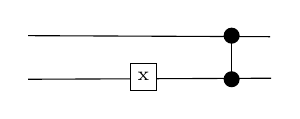
\begin{tikzpicture}[x=0.75pt,y=0.75pt,yscale=-1,xscale=1]
%uncomment if require: \path (0,300); %set diagram left start at 0, and has height of 300

%Straight Lines [id:da732813246379387] 
\draw    (99.83,109.67) -- (216.33,110.17) ;
%Straight Lines [id:da6605550224031504] 
\draw    (99.83,130.67) -- (216.83,130.17) ;
%Straight Lines [id:da2257066549092701] 
\draw    (197.83,109.67) -- (197.83,130.67) ;
\draw [shift={(197.83,130.67)}, rotate = 90] [color={rgb, 255:red, 0; green, 0; blue, 0 }  ][fill={rgb, 255:red, 0; green, 0; blue, 0 }  ][line width=0.75]      (0, 0) circle [x radius= 3.35, y radius= 3.35]   ;
\draw [shift={(197.83,109.67)}, rotate = 90] [color={rgb, 255:red, 0; green, 0; blue, 0 }  ][fill={rgb, 255:red, 0; green, 0; blue, 0 }  ][line width=0.75]      (0, 0) circle [x radius= 3.35, y radius= 3.35]   ;
%Shape: Rectangle [id:dp8096940990542667] 
\draw  [fill={rgb, 255:red, 255; green, 255; blue, 255 }  ,fill opacity=1 ] (149.3,123) -- (161.83,123) -- (161.83,136) -- (149.3,136) -- cycle ;

% Text Node
\draw (151.3,126) node [anchor=north west][inner sep=0.75pt]  [font=\tiny] [align=left] {{\scriptsize x}};


\end{tikzpicture}
    \caption{Circuit of two qubits being acted on by an X gate on the second, followed by a CZ gate over both.}
    \label{fig_APP:X - CZ }
\end{figure}

What we want to find then is the combination of X and Z matrices that gives us a matrix equivalent to $CZ(X\otimes\mathbb{I})$. We won't derive it here but we can easily show that $CZ(X\otimes\mathbb{I}) = (X\otimes Z)CZ$:

\begin{align} \label{eqn_APP: CZ commute X}
    CZ(X\otimes\mathbb{I}) & = 
    \begin{bmatrix}
        1 & 0 & 0 & 0 \\
        0 & 1 & 0 & 0 \\
        0 & 0 & 1 & 0 \\
        0 & 0 & 0 & -1 \\
    \end{bmatrix} \cdot
    \begin{bmatrix}
        0 & 0 & 1 & 0 \\
        0 & 0 & 0 & 1 \\
        1 & 0 & 0 & 0 \\
        0 & 1 & 0 & 0 \\
    \end{bmatrix}
    \\ & =
    \begin{bmatrix}
        0 & 0 & 1 & 0 \\
        0 & 0 & 0 & 1 \\
        1 & 0 & 0 & 0 \\
        0 & -1 & 0 & 0 \\
    \end{bmatrix}
    \\ & = 
    \begin{bmatrix}
        0 & 0 & 1 & 0 \\
        0 & 0 & 0 & -1 \\
        1 & 0 & 0 & 0 \\
        0 & -1 & 0 & 0 \\
    \end{bmatrix} \cdot
    \begin{bmatrix}
        1 & 0 & 0 & 0 \\
        0 & 1 & 0 & 0 \\
        0 & 0 & 1 & 0 \\
        0 & 0 & 0 & -1 \\
    \end{bmatrix} 
    \\ & = 
    \left(
    \begin{bmatrix}
        0 & 1 \\
        1 & 0 \\
    \end{bmatrix}
    \otimes
    \begin{bmatrix}
        1 & 0 \\
        0 & -1 \\
    \end{bmatrix}  \right) \cdot 
    \begin{bmatrix}
        1 & 0 & 0 & 0 \\
        0 & 1 & 0 & 0 \\
        0 & 0 & 1 & 0 \\
        0 & 0 & 0 & -1 \\
    \end{bmatrix} 
    \\ & = 
    (X\otimes\mathbb{Z})CZ
\end{align}

\begin{figure}
    \centering
    

\tikzset{every picture/.style={line width=0.75pt}} %set default line width to 0.75pt        

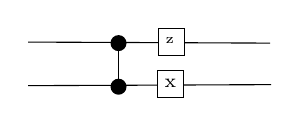
\begin{tikzpicture}[x=0.75pt,y=0.75pt,yscale=-1,xscale=1]
%uncomment if require: \path (0,300); %set diagram left start at 0, and has height of 300

%Straight Lines [id:da732813246379387] 
\draw    (99.83,109.67) -- (216.33,110.17) ;
%Straight Lines [id:da6605550224031504] 
\draw    (99.83,130.67) -- (216.83,130.17) ;
%Straight Lines [id:da2257066549092701] 
\draw    (143.33,110.17) -- (143.33,131.17) ;
\draw [shift={(143.33,131.17)}, rotate = 90] [color={rgb, 255:red, 0; green, 0; blue, 0 }  ][fill={rgb, 255:red, 0; green, 0; blue, 0 }  ][line width=0.75]      (0, 0) circle [x radius= 3.35, y radius= 3.35]   ;
\draw [shift={(143.33,110.17)}, rotate = 90] [color={rgb, 255:red, 0; green, 0; blue, 0 }  ][fill={rgb, 255:red, 0; green, 0; blue, 0 }  ][line width=0.75]      (0, 0) circle [x radius= 3.35, y radius= 3.35]   ;
%Shape: Rectangle [id:dp8096940990542667] 
\draw  [fill={rgb, 255:red, 255; green, 255; blue, 255 }  ,fill opacity=1 ] (162.3,123.5) -- (174.83,123.5) -- (174.83,136.5) -- (162.3,136.5) -- cycle ;
%Shape: Rectangle [id:dp33853823787750703] 
\draw  [fill={rgb, 255:red, 255; green, 255; blue, 255 }  ,fill opacity=1 ] (162.8,103) -- (175.33,103) -- (175.33,116) -- (162.8,116) -- cycle ;

% Text Node
\draw (164.3,126.5) node [anchor=north west][inner sep=0.75pt]  [font=\tiny] [align=left] {{\scriptsize x}};
% Text Node
\draw (164.8,106) node [anchor=north west][inner sep=0.75pt]  [font=\tiny] [align=left] {z};


\end{tikzpicture}

    \caption{Circuit where the CZ gate is applied over both qubits and then a Z gate is applied to the first whilst an X is applied to the second. This is equivalent to \ref{fig_APP:X - CZ }.}
    \label{fig_APP:CZ-X}
\end{figure}

This is equivalent to the CZ gate being applied across both qubits followed by a Z gate acting on the first qubit and an X gate acting on the second. This is diagrammatically shown in \ref{fig_APP:CZ-X}. It should be noted that these commutation relations for CZ gates and Pauli gates are symmetric across qubits so $CZ(\mathbb{I}\otimes X) = (Z\otimes X)CZ$\footnote{This equation means that an X on the first qubit followed by a CZ across both = a CZ gate followed by an X on the first and a Z on the second}.

\subsubsection{How CZ commutes with Z}
This is by far the easiest to understand and see. CZ and Z commute with each other without any need for correction. What we mean by this is $CZ(Z\otimes\mathbb{I}) = (Z\otimes\mathbb{I})CZ$ and thanks to the symmetry we just covered at the end of \ref{sec:CZ commute X} we know $CZ(\mathbb{I}\otimes Z) = (\mathbb{I}\otimes Z)CZ$. The 'proof' looks exactly like \ref{eqn_APP: CZ commute X}.

\subsubsection{How CZ commutes with XZ}
Now that we know how CZ commutes with the X gate and the Z gate we can take a look at how it commutes with an X gate followed by a Z (it is as an intuitive answer as we might expect).

\begin{figure}
    \centering

\tikzset{every picture/.style={line width=0.75pt}} %set default line width to 0.75pt        

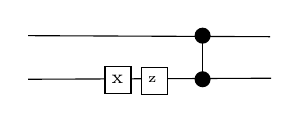
\begin{tikzpicture}[x=0.75pt,y=0.75pt,yscale=-1,xscale=1]
%uncomment if require: \path (0,300); %set diagram left start at 0, and has height of 300

%Straight Lines [id:da732813246379387] 
\draw    (99.83,109.67) -- (216.33,110.17) ;
%Straight Lines [id:da6605550224031504] 
\draw    (99.83,130.67) -- (216.83,130.17) ;
%Straight Lines [id:da2257066549092701] 
\draw    (183.83,109.67) -- (183.83,130.67) ;
\draw [shift={(183.83,130.67)}, rotate = 90] [color={rgb, 255:red, 0; green, 0; blue, 0 }  ][fill={rgb, 255:red, 0; green, 0; blue, 0 }  ][line width=0.75]      (0, 0) circle [x radius= 3.35, y radius= 3.35]   ;
\draw [shift={(183.83,109.67)}, rotate = 90] [color={rgb, 255:red, 0; green, 0; blue, 0 }  ][fill={rgb, 255:red, 0; green, 0; blue, 0 }  ][line width=0.75]      (0, 0) circle [x radius= 3.35, y radius= 3.35]   ;
%Shape: Rectangle [id:dp8096940990542667] 
\draw  [fill={rgb, 255:red, 255; green, 255; blue, 255 }  ,fill opacity=1 ] (136.8,124.5) -- (149.33,124.5) -- (149.33,137.5) -- (136.8,137.5) -- cycle ;
%Shape: Rectangle [id:dp33853823787750703] 
\draw  [fill={rgb, 255:red, 255; green, 255; blue, 255 }  ,fill opacity=1 ] (154.3,125) -- (166.83,125) -- (166.83,138) -- (154.3,138) -- cycle ;

% Text Node
\draw (138.8,127.5) node [anchor=north west][inner sep=0.75pt]  [font=\tiny] [align=left] {{\scriptsize x}};
% Text Node
\draw (156.3,128) node [anchor=north west][inner sep=0.75pt]  [font=\tiny] [align=left] {z};


\end{tikzpicture}

    \caption{Circuit of two qubits where the X and Z gates are applied to the second qubit (one after the other) followed by a CZ gate applied across both qubits}
    \label{fig_APP:XZ-CZ}
\end{figure}

We start with \ref{fig_APP:XZ-CZ} which can be represented as $CZ(Z\otimes\mathbb{I})(X\otimes\mathbb{I})$ and then we just apply the identities we showed above:
\begin{align}
    CZ(Z\otimes\mathbb{I})(X\otimes\mathbb{I}) = (Z\otimes\mathbb{I})CZ(X\otimes\mathbb{I}) =
    (Z\otimes\mathbb{I})(X\otimes Z)CZ
\end{align}

This right-hand side is shown in \ref{fig_APP:CZ-XZ}. As we've shown for other gates, the qubit symmetry applies here as well so we can say that $CZ(\mathbb{I}\otimes Z)(\mathbb{I}\otimes X) = 
    (\mathbb{I}\otimes Z)(Z\otimes X)CZ$
\begin{figure}
    \centering

\tikzset{every picture/.style={line width=0.75pt}} %set default line width to 0.75pt        

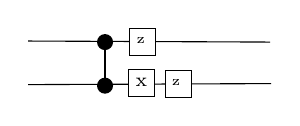
\begin{tikzpicture}[x=0.75pt,y=0.75pt,yscale=-1,xscale=1]
%uncomment if require: \path (0,300); %set diagram left start at 0, and has height of 300

%Straight Lines [id:da732813246379387] 
\draw    (99.83,109.67) -- (216.33,110.17) ;
%Straight Lines [id:da6605550224031504] 
\draw    (99.83,130.67) -- (216.83,130.17) ;
%Straight Lines [id:da2257066549092701] 
\draw    (136.83,110.17) -- (136.83,131.17) ;
\draw [shift={(136.83,131.17)}, rotate = 90] [color={rgb, 255:red, 0; green, 0; blue, 0 }  ][fill={rgb, 255:red, 0; green, 0; blue, 0 }  ][line width=0.75]      (0, 0) circle [x radius= 3.35, y radius= 3.35]   ;
\draw [shift={(136.83,110.17)}, rotate = 90] [color={rgb, 255:red, 0; green, 0; blue, 0 }  ][fill={rgb, 255:red, 0; green, 0; blue, 0 }  ][line width=0.75]      (0, 0) circle [x radius= 3.35, y radius= 3.35]   ;
%Shape: Rectangle [id:dp8096940990542667] 
\draw  [fill={rgb, 255:red, 255; green, 255; blue, 255 }  ,fill opacity=1 ] (148.3,123.5) -- (160.83,123.5) -- (160.83,136.5) -- (148.3,136.5) -- cycle ;
%Shape: Rectangle [id:dp33853823787750703] 
\draw  [fill={rgb, 255:red, 255; green, 255; blue, 255 }  ,fill opacity=1 ] (165.8,124) -- (178.33,124) -- (178.33,137) -- (165.8,137) -- cycle ;
%Shape: Rectangle [id:dp7489575253195708] 
\draw  [fill={rgb, 255:red, 255; green, 255; blue, 255 }  ,fill opacity=1 ] (148.8,103.5) -- (161.33,103.5) -- (161.33,116.5) -- (148.8,116.5) -- cycle ;

% Text Node
\draw (150.3,126.5) node [anchor=north west][inner sep=0.75pt]  [font=\tiny] [align=left] {{\scriptsize x}};
% Text Node
\draw (167.8,127) node [anchor=north west][inner sep=0.75pt]  [font=\tiny] [align=left] {z};
% Text Node
\draw (150.8,106.5) node [anchor=north west][inner sep=0.75pt]  [font=\tiny] [align=left] {z};


\end{tikzpicture}

    \caption{Circuit where the CZ gate is applied across 2 qubits, followed by an X gate applied to the second qubit and a pair of Z gates applied to both. This is equivalent to \ref{fig_APP:XZ-CZ}}
    \label{fig_APP:CZ-XZ}
\end{figure}

\subsubsection{How CZ commutes with 2 X gates}
Here we'll look at how the CZ gate commutes with two X gates applied across 2 qubits. This looks like \ref{fig_APP:XX-CZ}. The trick to finding the commutation relation here revolves around splitting up the tensor product. We start with $CZ(X\otimes X)$):
\begin{equation}
    CZ(X\otimes X) = CZ(X\otimes \mathbb{I})(\mathbb{I}\otimes X)
\end{equation}
and then just like before we commute CZ through the equation on the right-hand side:
\begin{align}
    CZ(X\otimes X) &=  CZ(X\otimes \mathbb{I})(\mathbb{I}\otimes X)
    \\ & = (X\otimes Z)CZ(\mathbb{I}\otimes X)
    \\ & = (X\otimes Z)(Z\otimes X)CZ
\end{align}


\begin{figure}
    \centering
\tikzset{every picture/.style={line width=0.75pt}} %set default line width to 0.75pt        

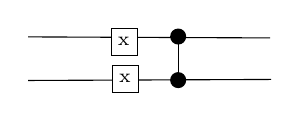
\begin{tikzpicture}[x=0.75pt,y=0.75pt,yscale=-1,xscale=1]
%uncomment if require: \path (0,300); %set diagram left start at 0, and has height of 300

%Straight Lines [id:da732813246379387] 
\draw    (99.83,109.67) -- (216.33,110.17) ;
%Straight Lines [id:da6605550224031504] 
\draw    (99.83,130.67) -- (216.83,130.17) ;
%Straight Lines [id:da2257066549092701] 
\draw    (172.07,109.5) -- (172.07,130.5) ;
\draw [shift={(172.07,130.5)}, rotate = 90] [color={rgb, 255:red, 0; green, 0; blue, 0 }  ][fill={rgb, 255:red, 0; green, 0; blue, 0 }  ][line width=0.75]      (0, 0) circle [x radius= 3.35, y radius= 3.35]   ;
\draw [shift={(172.07,109.5)}, rotate = 90] [color={rgb, 255:red, 0; green, 0; blue, 0 }  ][fill={rgb, 255:red, 0; green, 0; blue, 0 }  ][line width=0.75]      (0, 0) circle [x radius= 3.35, y radius= 3.35]   ;
%Shape: Rectangle [id:dp8096940990542667] 
\draw  [fill={rgb, 255:red, 255; green, 255; blue, 255 }  ,fill opacity=1 ] (140.3,123.5) -- (152.83,123.5) -- (152.83,136.5) -- (140.3,136.5) -- cycle ;
%Shape: Rectangle [id:dp4624452996610504] 
\draw  [fill={rgb, 255:red, 255; green, 255; blue, 255 }  ,fill opacity=1 ] (139.8,105.5) -- (152.33,105.5) -- (152.33,118.5) -- (139.8,118.5) -- cycle ;

% Text Node
\draw (142.3,126.5) node [anchor=north west][inner sep=0.75pt]  [font=\tiny] [align=left] {{\scriptsize x}};
% Text Node
\draw (141.8,108.5) node [anchor=north west][inner sep=0.75pt]  [font=\tiny] [align=left] {{\scriptsize x}};

\end{tikzpicture}
    \caption{Circuit where the X gate is applied across both qubits followed by the CZ gate applied across both}
    \label{fig_APP:XX-CZ}
\end{figure}

The right-hand side is shown in \ref{fig_APP:CZ - ZX,xZ}.

\begin{figure}
    \centering
\tikzset{every picture/.style={line width=0.75pt}} %set default line width to 0.75pt        

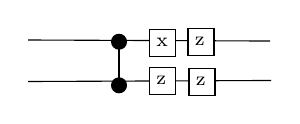
\begin{tikzpicture}[x=0.75pt,y=0.75pt,yscale=-1,xscale=1]
%uncomment if require: \path (0,300); %set diagram left start at 0, and has height of 300

%Straight Lines [id:da732813246379387] 
\draw    (99.83,110.67) -- (216.33,111.17) ;
%Straight Lines [id:da6605550224031504] 
\draw    (99.83,130.67) -- (216.83,130.17) ;
%Straight Lines [id:da2257066549092701] 
\draw    (143.57,111.5) -- (143.57,132.5) ;
\draw [shift={(143.57,132.5)}, rotate = 90] [color={rgb, 255:red, 0; green, 0; blue, 0 }  ][fill={rgb, 255:red, 0; green, 0; blue, 0 }  ][line width=0.75]      (0, 0) circle [x radius= 3.35, y radius= 3.35]   ;
\draw [shift={(143.57,111.5)}, rotate = 90] [color={rgb, 255:red, 0; green, 0; blue, 0 }  ][fill={rgb, 255:red, 0; green, 0; blue, 0 }  ][line width=0.75]      (0, 0) circle [x radius= 3.35, y radius= 3.35]   ;
%Shape: Rectangle [id:dp8096940990542667] 
\draw  [fill={rgb, 255:red, 255; green, 255; blue, 255 }  ,fill opacity=1 ] (177.3,124.5) -- (189.83,124.5) -- (189.83,137.5) -- (177.3,137.5) -- cycle ;
%Shape: Rectangle [id:dp4624452996610504] 
\draw  [fill={rgb, 255:red, 255; green, 255; blue, 255 }  ,fill opacity=1 ] (158.3,105.5) -- (170.83,105.5) -- (170.83,118.5) -- (158.3,118.5) -- cycle ;
%Shape: Rectangle [id:dp21808645132641424] 
\draw  [fill={rgb, 255:red, 255; green, 255; blue, 255 }  ,fill opacity=1 ] (158.3,124) -- (170.83,124) -- (170.83,137) -- (158.3,137) -- cycle ;
%Shape: Rectangle [id:dp008241843524475545] 
\draw  [fill={rgb, 255:red, 255; green, 255; blue, 255 }  ,fill opacity=1 ] (176.8,105) -- (189.33,105) -- (189.33,118) -- (176.8,118) -- cycle ;

% Text Node
\draw (179.3,127.5) node [anchor=north west][inner sep=0.75pt]  [font=\tiny] [align=left] {{\scriptsize z}};
% Text Node
\draw (160.3,108.5) node [anchor=north west][inner sep=0.75pt]  [font=\tiny] [align=left] {{\scriptsize x}};
% Text Node
\draw (160.3,127) node [anchor=north west][inner sep=0.75pt]  [font=\tiny] [align=left] {{\scriptsize z}};
% Text Node
\draw (178.8,108) node [anchor=north west][inner sep=0.75pt]  [font=\tiny] [align=left] {{\scriptsize z}};


\end{tikzpicture}
    \caption{2 Qubit Circuit where the CZ gate is applied across both qubits followed by an X and then Z on the first, and a Z then X on the second. This is equivalent to the circuit \ref{fig_APP:XX-CZ}}
    \label{fig_APP:CZ - ZX,xZ}
\end{figure}

\subsubsection{How CZ commutes with 2 XZ gate combinations}
We're going to skip all the other kinds of combinations that can be done with X and Z gates commuting with CZ and focus on how CZ commutes through an X and Z gate applied to both qubits. We start with $CZ(X\otimes X)(Z\otimes Z)$:
\begin{align}
    CZ(X\otimes X)(Z\otimes Z) & = (X\otimes Z)(Z\otimes X)CZ(Z\otimes Z)
    \\ & = (X\otimes Z)(Z\otimes X)(Z\otimes Z)CZ
\end{align}
We can then simplify this using the fact that $X \cdot X \equiv \mathbb{I}$ and $Z \cdot Z \equiv \mathbb{I}$:

\begin{align}
    CZ(X\otimes X)(Z\otimes Z) & = (X\otimes Z)(Z\otimes X)(Z\otimes Z)CZ
    \\ & = (X\otimes Z)(Z\otimes\mathbb{I})(\mathbb{I}\otimes X)(Z\otimes\mathbb{I})(\mathbb{I}\otimes Z)CZ
    \\ & = (X\otimes Z)(\mathbb{I}\otimes X)(Z\otimes\mathbb{I})(Z\otimes\mathbb{I})(\mathbb{I}\otimes Z)CZ \label{qubit order swap}
    \\ & = (X\otimes Z)(\mathbb{I}\otimes X)(\mathbb{I}\otimes Z)CZ
\end{align}
where in \ref{qubit order swap} we use the fact that $(Z\otimes\mathbb{I})$ commutes with $(\mathbb{I}\otimes X)$ since these are single qubit gate operators acting on different qubits.
\par
What makes this result interesting is that because the left-hand side of the above equation is symmetric, our result is equal to its qubit symmetric pair. Meaning that:
\begin{equation}
     CZ(X\otimes X)(Z\otimes Z) = (X\otimes Z)(\mathbb{I}\otimes X)(\mathbb{I}\otimes Z)CZ = (Z\otimes X)(X\otimes \mathbb{I})(Z\otimes \mathbb{I})CZ
\end{equation}
% \begin{center}
%     \Huge \textbf{Old notes and scrap space}
% \end{center}
% \vspace{-1em}

% \section{Jans notes}
Ok, I'm taking over this section for now
\begin{itemize}

\item
For "types" fo QCters I see photonic and trapped ion for now at least.

\item
Trapped ion type seems quite nice, apparently it works well, but they haven't really scaled to hundreds of qubits.


\item
Found this thing called DiVincezo criteria which might be nice to mention or something, it's 5 criteria that need to be met for a given
hypothetical QCter type/implementation:
\begin{itemize}
    \item A physical system containing well-defined 2 level quantum systems (qubits) which can be isolated from the environment.
    \item The ability to initialize this system in a well defined, determinate state.
    \item A set of universtal quantum gates which can be applied to each qubit or possibly pairs (or more) of them.
    \item Qubit decoherence times much greater than times for quantum gates to be applied.
    \item The ability to read out qubit state with high accuracy.
    \item ** In addition 2 more were mentioned by him, the ability to convert between "stationary" (like trapped ions) and "flying" (photons) states which would be necessary for a quantum network.
\end{itemize}

\item Trapped ion systems, kinda taken from Bruzewicz 2019, they also mention the DiVincezo stuff
\begin{itemize}
    \item The actual states are the electronic states of some atom/ion.
    \item A couple types: hyperfine, Zeeman, fine structure and optical the differences between them is the particular energy levels that are used for states.
            The names make it decently clear, fine structure means the fine structure split states are used, optical means states which are transitioned between by photon emission/absorption.
    \item One of the things to deal with is that the atoms energies come from both their structure and their motion within the trap (which is also quantized).
    \item Some of the manipulations take place through lasers.
    \item Main pros are long coherence time and great gate and initialization/readout fidelity, drawbacks include speed, the gates are quite slow compared to other qubit technologies.
    \item Unordered random facts
    \begin{itemize}
        \item single qubit gates take a couple micro seconds and double about 10-100 micro seconds
        \item coherence times range from 0.2 to 600s (600s achieved for hyperfine) and surface code error correction was mentioned, the gate fielity should be good enough for that
        \item with respect to the optional DiVincezo, ions are unlikely to be the "flying" ones even though they can be moved, however high-fielity entanglement between ions and photons has been showed.
        \item most of the main things have been demonstrated by 2004 though the maximum number of ions achieved in a register so far was 20.
    \end{itemize}
\end{itemize}

\end{itemize}



% \section{Michael's Section}
Finding a physical representation of qubits that fulfil all the mathematical requirements is not easy.
Gaining control over a single quantum system has been a want since about 1970. word this so better
It is possible to see quantum effects on a vast number of combined quantum systems such as in superconductors. \cite{nielsen_quantum_2010}
Or in particle collisions again quantum effects are observed however there isn't control over a single quantum system.
Qubits are the physical realisation of controlling a single quantum system and its state.
You require a system with many degrees of freedom that can encode quantum information (qubits). \cite{bergou_quantum_2021}

\subsection{Optical Photon Quibit}

{\bf Why Photons?}
\begin{itemize}
    \item Photons are massless, chargeless and don't interact with each other or other mass much. \cite{nielsen_quantum_2010}
    \item Can be guided long distances without much energy loss using optical fibers. \cite{nielsen_quantum_2010}
    \item Quantum information can be transmitted over long distances using photons as demonstrated by quantum entanglement over 1200km. \cite{yin_satellite-based_2017}
    \item photons can maintain entanglement over long distances and time period allowing the transmission quantum information. - this supper secure wow \cite{thibault_team_nodate}
\end{itemize}

\vspace{1em}
{\bf How photons?}

\begin{itemize}
    \item The transverse polarisation state of a photon can be used to represent qubits. 
    These are vertical, horizontal linear and left, right circular polarization. \cite{bergou_quantum_2021}
    
    \item These states can also be maintained - in isotropic materials photons polarization does not change as it propagates. \cite{bergou_quantum_2021}
    
    \item $\left\vert 0 \right\rangle = \left\vert H\right\rangle $ and $\left\vert 1 \right\rangle = \left\vert V\right\rangle $ where H and V are horizontal and vertical polarisation. \cite{bergou_quantum_2021}

\end{itemize}
\vspace{1em}
{\bf Need a single photon source}
\begin{itemize}
    \item lasers with very low output can emit single electrons... but 90$\%$ of the time no photon is emitted and when there is a photon emitted 5$\%$ of than one is emitted.\cite{nielsen_quantum_2010}
    \begin{itemize}
        \item so lasers CANNOT be used - we need sources that can be synchronised not possible if you don't know when a photon is actual coming out
    \end{itemize}
\end{itemize}
\vspace{1em}
{\bf Quantum Dot}
\begin{itemize}
    \item Quantum dots can (kinda) be a single photon source
    \item from wiki quantum dots seem to be `semiconducting particles a few nanometers in size' therefor shining light on it would emit one photon is the idea
    \item need to understand $T_1$ and $T_2$ coherance times.... think $T_2$ is the time taken for the inital and final states to be uncorrelated (i.e. $|1\rangle \rightarrow \alpha |0\rangle + \beta |1\rangle$ a liner combination of them both?
    \item anyway... using a narrow-linewidth laser which had the same resonance as the quantum dot single photon emission was achieved with a $T_2=22ns$ (apparently long) was achieved. \cite{lodahl_interfacing_2015}
\end{itemize}
\vspace{1em}
{\bf DiVincenzo Criteria} \cite{bergou_quantum_2021}
\begin{itemize}
    \item Scalability with well defined qubits
    
    \begin{itemize}
        \item $\left\vert 0 \right\rangle = \left\vert H\right\rangle $ and $\left\vert 1 \right\rangle = \left\vert V\right\rangle $ where H and V are horizontal and vertical polarisation.  
        \item polarisation state can be maintained for a long time
        \item or timebin/path encoding \cite{obrien_optical_2007}

        \item eventually need like $10^{11}$ single photon states. posible way of doing this is using $10^11$ sources that can reliably produce a photon as in when requested
        \begin{itemize}
            \item don't exist yet, but are being worked on some promising are quantum dots, trapped ions and atoms, color centers in diamonds, semiconductors \cite{slussarenko_photonic_2019}
        \end{itemize}
    \end{itemize}

    \item Initializing qubits to a simple fiducial state
    \begin{itemize}
        \item quantum dot - single photon source. when excited on resonance by low laser prob of emmiting two photons instead of one is super low \cite{santori_indistinguishable_2002}
    \end{itemize}

    \item  A qubit-specific measurement capability
    \begin{itemize}
        \item an ideal photon detector which detects every individual photon with no dark count (false positive) doesn't yet exist. 
        \item one of the most used detectors currently is the Si avalanche photodiode... only has a detection efficiency of 65$\%$! so the probability of detecting 10 photons with 10 detectors is less than $2\%$. \cite{slussarenko_photonic_2019}
        \item better now we have superconducting nanowire single-photon detectors (SNSPDs) with reset rate $\sim$40ns and detection efficiency $>95\%$ ... but these need temos of around 2K. \cite{santori_indistinguishable_2002}
        
    \end{itemize}
    
    \item Long relevant decoherence times
    \begin{itemize}
        \item 
    \end{itemize}

    \item A ``universal'' set of quantum gates
    \begin{itemize}
        \item birefringent wave plates for one qubit gates \cite{obrien_optical_2007}
    
        \item deeterministic CNOT gates difficult (these are the double qubit ones). A 2007 paper suggests that for a near deterministic CNOT gate (i.e. not deterministic just low prob) it requires $>$10 000 entangled photons for only $>95\%$ success probability \cite{obrien_optical_2007}
    \end{itemize}

    \item The ability to interconvert stationary and flying qubits
    \begin{itemize}
        \item can use polarizing beam splitters to convert between polarisation and path encoding \cite{obrien_optical_2007}
    \end{itemize}

    \item The ability to transmit flying qubits between specified locations
    \begin{itemize}
        \item well photons are transmitted all the time!
        \item actually kind of difficult cause photons are always 'flying' so some kind of optical quantum memory may be necesarry to store them. 
    \end{itemize}
\end{itemize}

% \section{Summary}
Studies of the nuclear force are a fascinating yet unfinished part of physics.
Though most simple interactions involving it are well understood, it is yet to be applied to more complicated systems.
Mass spectrometers have been crucial in testing nuclear theories and pushing their limits.
They have allowed for the exploration of the nuclear landscape closer to the neutron dripline where models using only 2N interactions have been insufficient in predicting the shell closures of these exotic nuclei.
Future MS such as the PENTATRAP experiment or the many MR-TOF spectrometers that are being developed, with improved resolving power and shorter needed observation time will be crucial in probing and improving the leading nuclear force theories.

% \section{Pablo's notes}

To effectively perform quantum computation it is necessary to be able to manipulate qubits and perform unitary operations on them. Furthermore, any unitary transformation can be composed of single qubit operations and CNOT gates. Thus, an experimental quantum computer should be able to implement them appropriately.

\subsection{Optical Photon Quantum Computer}

The correct combination of phase shifters and beam splitters allow the creation of any single qubit gate. This is a consequence of the theorem that states that any single qubit operation can be generated from z and y-axis rotations. A phase shifter performs $R_{z}$ rotations and a beamsplitter performs $R_{y}$ rotations.

Nonlinear Kerr media allow for the creation of a two qubit gate. The main experimental problem with this setup is succesfully making two photons interact. The available nonlinear Kerr media today cannot reliably obtain the $\pi$ cross phase modulation necessary to implement a CNOT gate. 

\subsection{Optical cavity quantum electrodynamics}

The main idea behind this model is the question of whether the state of a photon can be transferred to and from single atoms, whose interactions would be easier to control. Single qubit operations are constructed in the same way as in the optical photon quantum computer.

The CNOT gate can be implemented by coupling atoms enclosed in a Fabry-Perot cavity to the optical field of the photons.

\subsection{Ion Trap}

Have to talk it over. Have not managed to fully understand how quantum gates would be constructed in this setup.

\subsection{Nuclear Magnetic Resonance}

The main difference with this method compared to the previous is that we are acting on an ensemble of particles. Arbitrary single qubit transforms can be constructed from magnetic field pulses applied to spins in a strong magnetic field. Coupling between the molecules and, thus, the realization of a two qubit gate can be provided by chemical bonds between neighbouring atoms.

% \section{Matthew's notes}

\subsection{What are registers?}
Registers are a form of memory for data instantaneously in use by the CPU (https://www.javatpoint.com/computer-registers). Any data that the CPU wants to process must first be stored in a register. Fundamentally, a register is a group of flip-flops which can each store a bit of data. 

Give an example of a register..
Explain what a flip flop is..

\subsection{Quantum Registers}
Quantum registers are analogous to classical registers because they store the data that is processed by the computer. 

Rather than a group of flip-flop circuits, it is a superposition of qubits. A classical register can store one of $2^n$ different values for $n$ flip-flops. By comparison, a quantum register of $n$ qubits can store all $2^n$ values simultaneously (https://cds.cern.ch/record/383367/files/p165.pdf). A quantum computer will require multiple registers for true computation (https://arxiv.org/pdf/quant-ph/9802065), for example by adding the contents of two registers together.

\subsection{Why use QCs?}
Originally proposed by Richard Feynman to solve quantum mechanics problems, these computers will be useful for molecular simulation which can be used for drug development. Particularly good for financial calculations which involve a lot of combinatorics (https://epjquantumtechnology.springeropen.com/articles/10.1140/epjqt/s40507-021-00091-1). Financial institutions will also be able to afford high investment into QC development. Typical programs use Monte Carlo simulation of market movements. Goldman Sachs is one example

\begin{itemize}

\item Explain why combinatorics problems are easily solved
\item Could talk more about Monte Carlo
\item Weather forecasting
\item https://learn.microsoft.com/en-us/azure/quantum/concepts-overview
\item https://medium.com/@markus.c.braun/a-brief-history-of-quantum-computing-a5babea5d0bd
\end{itemize}
Quantum computers have the potential to break much of today's encryption, particularly RSA which is based on prime factorisation. However, they also open the door to modern cryptography, such as quantum key distribution (QKD) which is theoretically unbreakable by laws of Physics rather than just mathematically difficult to solve.

\subsection{Why not to use QCs}
Although quantum computers have the potential to allow for many of the breakthroughs described above, they will not replace classical ones. Instead, both systems are likely to coexist. Many of the things that an average user uses a computer for could not be enhanced to for any practical benefit by a quantum computer. There is some classical computation that could in fact be much slower on a quantum machine due to all the extra overheads required to run one. Streaming video or writing documents involves a certainty in the data, if you press a key on the keyboard there is no ambiguity in what to store that as internally. Therefore, there is no need to consider all possibilities when doing day to day computation (https://ieeexplore.ieee.org/stamp/stamp.jsp?tp=&arnumber=8322045).

\subsection{Major Breakthroughs}
\begin{itemize}
    \item 1998 - first demonstration of two qubit system (https://semanticscholar.org/paper/6c055053f4f1605fdc0bd474c7a350dcd01f627d)
    \item 2019 - google declares quantum supremacy by performing a series of operations in 200 seconds that would take a supercomputer about 10,000 years to complete; IBM responds by suggesting it could take 2.5 days instead of 10,000 years, highlighting techniques a supercomputer may use to maximize computing speed (https://www.forbes.com/sites/gilpress/2021/05/18/27-milestones-in-the-history-of-quantum-computing/?sh=2506dc67b23f)
    \item 2021, IBM eagle which is 127 bit quantum processor. First QC which is so complex that it cannot be simulated reliably by a classical computer 'the number of classical bits necessary to represent a state on the 127-qubit processor exceeds the total number of atoms in the more than 7.5 billion people alive today' (https://newsroom.ibm.com/2021-11-16-IBM-Unveils-Breakthrough-127-Qubit-Quantum-Processor)
\end{itemize}


% \newpage

\end{document}
